
%(BEGIN_QUESTION)
% Copyright 2006, Tony R. Kuphaldt, released under the Creative Commons Attribution License (v 1.0)
% This means you may do almost anything with this work of mine, so long as you give me proper credit

A double-acting hydraulic cylinder has 500 PSI of pressure applied to the side without the rod and 750 PSI of pressure applied to the rod-side.  Calculate the resultant force generated at the piston and transmitted through to the rod, and also determine this force's direction.  The piston is 5 inches in diameter, and the rod is 1 inch in diameter.

$$\includegraphics[width=15.5cm]{i00156x01.eps}$$

\vskip 20pt \vbox{\hrule \hbox{\strut \vrule{} {\bf Suggestions for Socratic discussion} \vrule} \hrule}

\begin{itemize}
\item{} Identify which fundamental principles of science, technology, and/or math apply to each step of your solution to this problem.  In other words, be prepared to explain the reason(s) ``why'' for every step of your solution, rather than merely describing those steps.
\item{} What would happen if fluid pressure were applied to the bottom port and a fluid {\it vacuum} were applied to the top port?  Would this generate more force, less force, or the same amount of force as if the same fluid pressure were applied to bottom port and the top port left vented?
\item{} Would the piston experience a resultant force if both ports were connected together with a length of tubing (made ``common'' to each other) and then pressurized with the exact same amount of fluid pressure?  Why or why not?
\item{} Suppose both ports of this cylinder were connected together with a length of tubing (made ``common'' to each other) and to a pressure gauge.  What would that gauge register if the piston were then pushed in the downward direction?  Would the gauge's reading increase, decrease, or remain the same?  Explain your answer in detail.
\end{itemize}

\underbar{file i00156}
%(END_QUESTION)





%(BEGIN_ANSWER)

Net force = {\bf 4,319.69 pounds}, in the downward direction.

\vskip 10pt

If your calculated force turned out to be 4,908.7 pounds, you made a very common error.  Once you have figured out what this error is, go back and try to see how the scenario would have to be altered in order to actually generate 4,908.7 pounds of force with the two pressures being 750 PSI and 500 PSI, respectively.

%(END_ANSWER)





%(BEGIN_NOTES)

In this scenario, there are two pressures fighting against each other: the 750 PSI pressure is pressing downward on the piston while the 500 PSI pressure is pressing upward.  The force calculation is complicated by the fact that the two pressures are not acting against equal surface areas.  The upper pressure has to act on a smaller piston area, because the rod ``shields'' part of the upper piston surface from the 750 PSI fluid pressure. 

\vskip 10pt

Area of piston bottom:

$$A = \pi r^2 = \pi \left(5 \hbox{ in} \over 2 \right)^2 = 19.635 \hbox{ in}^2$$

Effective area of piston top:

$$A = \pi r_1^2 - \pi r_2^2 = \pi \left(5 \hbox{ in} \over 2 \right)^2 - \pi \left(1 \hbox{ in} \over 2 \right)^2 = 19.635 \hbox{ in}^2 - 0.7854 \hbox{ in}^2 = 18.850 \hbox{ in}^2$$

\vskip 30pt

Force up:

$$F = PA = (500 \hbox{ PSI}) (19.635 \hbox{ in}^2) = 9817.47 \hbox{ lb (up)}$$

\vskip 10pt

Force down:

$$F = PA = (750 \hbox{ PSI}) (18.850 \hbox{ in}^2) = 14137.17 \hbox{ lb (down)}$$

\vskip 10pt

Resultant force:

$$14137.17 \hbox{ lb} - 9817.47 \hbox{ lb} = 4319.69 \hbox{ lb (down)}$$

%INDEX% Physics, fluids: pressure, force, and area

%(END_NOTES)


